\documentclass{article}
\usepackage[utf8]{inputenc}
\usepackage{tikz}

\begin{document}
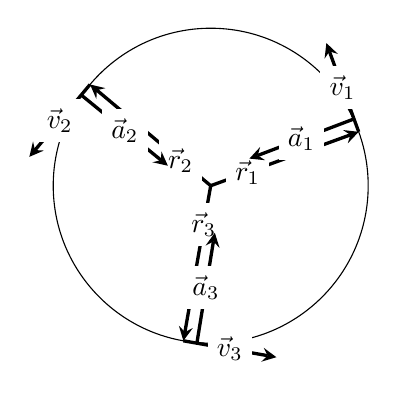
\begin{tikzpicture}[scale=2,>=stealth]

%Draw Circle radius 1 cm
	\draw (0,0) circle (1cm);
	
%The foreach command counts the angle of the distance vectors and which distance vector
	\foreach \angle/\count in {20/1,140/2,260/3}
		{

%Draws the 3 distance vectors
		\draw [name=distance vectors,very thick,->] (0,0) -- node[near start,fill=white] {$\vec{r}_{\count}$} (\angle:1cm);
		
%Draws the 3 velocity vectors at right angles to the distance vectors
		\draw [name=velocity vectors,rotate around={90:(\angle:1cm)},very thick,->] (\angle:1cm) -- node[fill=white] {$\vec{v}_{\count}$} (\angle:1.6cm) ;
		
%Draws the 3 acceleration vectors directed inward and offset slightly from the distance vectors
		\draw [name=acceleration vectors,very thick,->] (\angle+5:1cm) -- node[fill=white] {$\vec{a}_{\count}$} (\angle+15:0.3cm) ;
	}

\end{tikzpicture}
\end{document}
